\documentclass[../main/main.tex]{subfiles}

\newdate{date}{0}{1}{2020}


\begin{document}


\chapter{Spontaneous symmetry breaking}

\marginpar{ \textbf{Lecture n.} \\  \displaydate{date}. \\ Compiled:  \today.}

\section{Spontaneous symmetry breaking}

When we talk about a broken symmetry, we often refer to a situation as
\begin{equation*}
  \mathcal{H} = \mathcal{H}_0 + \mathcal{H}_1
\end{equation*}
where \( \mathcal{H}_0 \)  is invariant under the group \( \mathcal{G} \) and \( \mathcal{H}_1 \) is invariant under a subgroup \( \mathcal{G}' \subset  \mathcal{G}\).

\begin{example}{Ising with magnetic field}{}
  Let us consider the Hamiltonian for the Ising model with a magnetic field \( H \neq 0 \):
\begin{equation*}
  \mathcal{H} = J \sum_{\expval{ij} }^{} S_i S_j + \sum_{i}^{} H_i S_i
\end{equation*}
The second term, \( \sum_{i}^{}  H_i S_i \), breaks the \( \mathbb{Z}^2 \) symmetry satisfied by the first alone.
\end{example}

\begin{example}{Hydrogen atom with an external field}{}
  An example, in quantum mechanics, is the hydrogen atom in presence of an electric field \( \va{E} \) (Stark effect) or a magnetic one, \( \va{B} \), (Zeeman effect). If \( \mathcal{H}_1 \) is small, the original symmetry is weakly violated and perturbative approaches are often used.
\end{example}

In all the above examples, one says that the symmetry is broken explicitly.

\begin{definition}{Spontaneous symmetry breaking}{}
The Hamiltonian maintains the original symmetry but the variables used to describe the system become asymmetric.
\end{definition}

At this point it is convenient to distinguish between
\begin{itemize}
\item \textbf{Discrete symmetries}: for instance \( \mathbb{Z}^2 \), \( \mathbb{Z}_q \).
\item \textbf{Continuous symmetries}: for instance \( XY \), \( O(n) \).
\end{itemize}

Let us consider first the discrete ones by focusing on the \( \mathbb{Z}^2 \) symmetry (Ising).
As previously said, if \( H=0 \), the Hamiltonian of the Ising model, \( \mathcal{H}_{\text{Ising}} \), is invariant with respect to the change \( S_i \rightarrow -S_i \), hence the discrete group is
\begin{equation*}
  \mathcal{G} = \mathbb{Z}^2
\end{equation*}
A Ginzburg-Landau theory of the Ising model is given by
\begin{equation}
   \beta \mathcal{H} (\Phi ) = \int_{}^{} \dd[d]{\va{x}} \qty[ \frac{1}{2} \qty(\va{\grad } \Phi )^2 + \frac{r_0}{2} \Phi ^2 + \frac{u_0}{4} \Phi ^4 - h \Phi ]
  \label{eq:n_4}
\end{equation}
Hence, the partition function can be computed as:
\begin{equation}
  Z (r_0,u_0,h) = \int_{}^{} \mathcal{D} [\Phi]  e^{-\beta \mathcal{H} (\Phi )}
  \label{eq:n_5}
\end{equation}
If we have \( h=0 \), the symmetry is \( \Phi \rightarrow - \Phi  \).
The equation of state obtained with saddle point approximation is
\begin{equation*}
  h = - \va{\grad } ^2 \Phi + r_0 \Phi + u_0 \Phi ^3
\end{equation*}
If \( h \) does not depend on \( \va{x} \), i.e. \( h(\va{x})=h \), the last equation reduces to the equation of state of the Landau theory of uniform system:
\begin{equation*}
  h =  r_0 \Phi + u_0 \Phi ^3
\end{equation*}

Let us remind that the saddle point appriximation constists in approximating the functional integral of Eq.\eqref{eq:n_5} with its dominant term, i.e. with the one for which the exponent (Eq.\eqref{eq:n_4}) is minimum. Therefore, in the uniform case (namely \( \va{\grad } \Phi = 0 \)), it is equivalent to find the uniform value \( \Phi _0 \)  that is the extrema of the potential:
\begin{equation*}
  V (\Phi ) = \frac{1}{2} r_0 \Phi ^2 + \frac{u_0}{4} \Phi ^4 - h \Phi
\end{equation*}
Hence, if \( h=0 \), the extrema of the potential can be computed as
\begin{equation*}
  V' = (r_0 + u_0 \Phi ^2) \Phi = 0
\end{equation*}

\begin{figure}[h!]
\begin{minipage}[c]{0.5\linewidth}
\subfloat[][Plot of the potential \( V (\Phi ) \) in the case \( r_0 > 0 \), i.e. \( T>T_c \).]{ 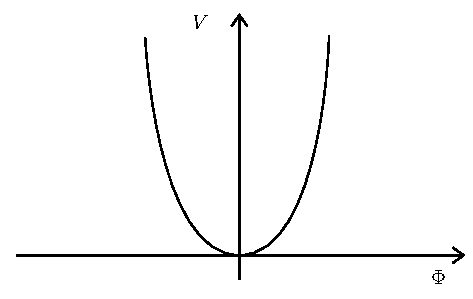
\includegraphics[width=0.8\textwidth]{../lessons/n_image/1.pdf}  \label{fig:n_5} }
\end{minipage}
\begin{minipage}[]{0.5\linewidth}
\centering
\subfloat[][Plot of the potential \( V (\Phi ) \) in the case \( r_0 < 0 \), i.e. \( T<T_c \).]{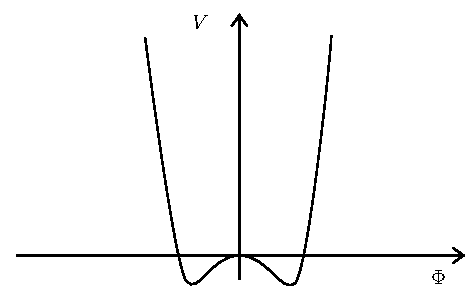
\includegraphics[width=0.8\textwidth]{../lessons/n_image/2.pdf}  \label{fig:n_6} }
\end{minipage}
\caption{\label{fig:} }
\end{figure}


Let us remember that \( r_0 \propto (T-T_c) \). In order to find the extrema of the potential \( V(\Phi ) \), we should distinguish two cases:

\begin{enumerate}
\item Case \( r_0>0 \) \( (T>T_c) \): there is only one solution \( \Phi _0 =0 \), as we can see in Figure \ref{fig:n_5}.

\item Case \( r_0<0 \) \( (T<T_c) \): there are two solutions \( \Phi _0 = \pm \sqrt{-\frac{r_0}{u_0}}  \), as illustrated in Figure \ref{fig:n_6}.

We note that the two solution \( \pm \Phi _0 \) are related by the \( \mathbb{Z}^2 \) transformation, namely \( \Phi \rightarrow - \Phi  \).
Moreover, in this case with \( T < T_c \), the two states (phases) \( \pm \Phi _0 \) have a lower symmetry than the state \( \Phi _0 = 0 \).

If the thermal fluctuations \( \delta \Phi  \) are sufficiently strong to allow passages between the two states \( \pm \Phi _0 \) at \( T < T_c \), we have \( \expval{\Phi } = 0  \) (preserves states).


However, for \( T < T_c \) and \( N \rightarrow + \infty  \), transition between the two states will be less and less probable and the system will be trapped into one of the two states \( (\pm \Phi _0) \). In other words, the system choose spontaneously one of the two less symmetric state. Therefore, its physics is not any more described by \( \Phi  \) but by the fluctuations \( \delta \Phi  \) around the chosen minimum \( \Phi _0 \). There is a spontaneous symmetry breaking. It means that the variable \( \Phi  \) is not any more symmetric and one has to look at \( \Phi \rightarrow \Phi _0 + \delta \Phi  \), where \( \delta \Phi  \) is a new variable!

\end{enumerate}





\section{Spontaneous breaking of continuous symmetries and the onset of Goldstone particles}
Let us start with a simple model in which the order parameter is a scalar complex variable
\begin{equation*}
  \Phi = \frac{\Phi _1 + i \Phi _2}{\sqrt{2} }
\end{equation*}
and with an Hamiltonian \( \mathcal{H} \) that is invariant with respect to a global continuous transformation. For instance, the simplest model in statistical mechanics that is invariant with respect to a continuous symmetry is the XY model with \( O(2) \) symmetry, or a Ginzburg-Landau model for a superfluid or a superconductor (with no magnetic field). Hence, we suppose that the Hamiltonian as the following form:
\begin{equation*}
  \beta \mathcal{H}_{eff} = \int_{}^{} \dd[d]{\va{x}} \qty[ \frac{1}{2} \va{\grad }\Phi \vdot \va{\grad } \Phi ^* + \frac{r_0}{2} \Phi  \Phi^* + \frac{u_0}{4} \qty(\Phi \Phi^* )^2 ]
\end{equation*}
where
\begin{equation*}
  \Phi (\va{x}) = \frac{1}{\sqrt{2} } \qty[ \Phi _1 (\va{x}) + i \Phi _2 (\va{x})], \quad \text{or} \quad \Phi (\va{x}) = \psi (\va{x}) e^{i \alpha (\va{x})}
\end{equation*}
The physical meaning of \( \Phi  \) depends on the case considered. If we have:

\begin{itemize}
\item Superfluid: \( \Phi  \) is the macroscopic wave function of the Bose condensate (density of superfluid \( n= \abs{\Phi ^2}  \)).
\item Superconductor: \( \Phi  \) is the single particle wave function describing the position of the centre of mass of the Cooper pair.
\end{itemize}

\subsection{Quantum relativistic case (field theory)}
In quantum mechanics the analog of the Hamiltonian \( \mathcal{H} \) is the action
\begin{equation}
  S(\Phi ) = \int_{}^{} \dd[4]{\va{x}}   \mathcal{L} ( \Phi )
\end{equation}
where
\begin{equation}
  \mathcal{L} (\Phi ) = - \frac{1}{2} \partial_\mu \Phi \partial^\mu \Phi ^*
  - \frac{r_0}{2} \Phi \Phi ^* - \frac{u_0}{4} \qty(\Phi \Phi ^*)^2
  \label{eq:n_8}
\end{equation}
The Lagrangian \( \mathcal{L} (\Phi ) \) describes a scalar complex (i.e. charged) \emph{muonic field} with mass \( m \equiv \sqrt{r_0} \); we note that, if  \( \mathcal{L} (\Phi ) \) describes a muonic field, we should have \( r_0>0 \) to have the mass \( m \) well defined. Moreover, the term \( (\Phi \Phi ^*)^2 \) means self-interaction with strenght \( \lambda \equiv u_0 \).

In all cases (\( r_0 > 0 \) or \( r_0 < 0 \)), the original symmetry is \( U(1) \); it means that both the Hamiltonian \( \mathcal{H} \) and the Lagrangian \( \mathcal{L} \) are invariant with respect to the transformation
\begin{equation}
  \Phi \rightarrow e^{i \theta } \Phi , \quad \Phi ^* \rightarrow e^{-i \theta } \Phi ^*
\end{equation}
where the phase \( \theta  \) does not depend on \( \va{x} \) (global symmetry).
In components the transformation becomes
\begin{equation*}
  \begin{cases}
   \Phi _1 \rightarrow  \Phi _1 \cos \theta - \Phi _2 \sin \theta \\
  \Phi _2 \rightarrow  \Phi _2 \cos \theta + \Phi _1 \sin \theta
  \end{cases}
  \quad \Rightarrow
  (\Phi _1', \Phi _2') = \begin{pmatrix}
  \cos \theta    & - \sin \theta   \\
    \sin \theta  & \cos \theta
  \end{pmatrix}
  \begin{pmatrix}
  \Phi _1 \\
  \Phi _2
  \end{pmatrix}
\end{equation*}

Now, let us focus first on the statistical mechanics model and to the most interesting case of \( r_0 <0 \).
In components, \( \mathcal{H} \) can be expressed as

\begin{equation}
  \beta \mathcal{H} = \int_{}^{} \dd[d]{\va{x}} \qty[\qty(\grad \Phi _1)^2 + \qty(\grad \Phi _2)^2  ] + \int_{}^{} \dd[d]{\va{x}} V (\Phi _1, \Phi _2)
\end{equation}
where the potential is
\begin{equation}
  V (\Phi _1, \Phi _2) = \frac{r_0}{2} \qty(\Phi _1^2 + \Phi _2^2) + \frac{u_0}{4} \qty( \Phi _1^2 + \Phi _2^2)^2
  \label{eq:n_6}
\end{equation}
In the case \( r_0 < 0 \), it is called \emph{mexican hat potential} and it is shown in Figure \ref{fig:n_1}.

\begin{figure}[h!]
\centering
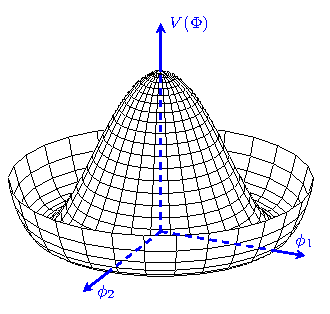
\includegraphics[width=0.6\textwidth]{../lessons/n_image/3.pdf}
\caption{\label{fig:n_1} Case \( r_0 < 0 \). The potential \( V(\Phi ) \) is a mexican hat potential.}
\end{figure}

In the uniform case we have \( (\grad \Phi _1 = \grad \Phi _2 = 0) \). Let us define
\( S = \sqrt{\Phi _1^2 + \Phi _2^2}  \), the potential in Eq.\eqref{eq:n_6} can be rewritten as:
\begin{equation*}
  V (S) = \frac{r_0}{2} S^2 + \frac{u_0}{4} S^4
\end{equation*}
In the uniform case, the solution is given by the minima of the potential \( V(S) \); hence, in order to find the extrema points, we derive the potential with respect to \( S \) and we impose the condition \( V'=0 \):
\begin{equation*}
  \dv{V(S)}{S} = r_0 S + u_0 S^3 = 0
\end{equation*}
We have a maximum at \( S=0 \) and a minimum at  \( S^2 \equiv v^2 = -  r_0/u_0 \). Hence, for \( r_0 < 0 \), the Hamiltonian \( \mathcal{H} \) displays a minimum when
\begin{equation*}
  \Phi _1^2 + \Phi _2^2 \equiv v^2 = - \frac{r_0}{u_0}
\end{equation*}
It could be represented in the \( 2d \) plane \( (\Phi _1, \Phi _2) \), where the minimum lies on a circle of radius
\begin{equation*}
  v = \sqrt{- \frac{r_0}{u_0}}
\end{equation*}
as show in Figure \ref{fig:n_4}.
The spontaneous symmetry breaking occurs when the system "chooses" one of the infinite available minima.
In our example, let us suppose that the chosen minimum is
\begin{equation}
  \Phi _1 = v = \sqrt{- \frac{r_0}{u_0}}, \quad \Phi _2 = 0
  \label{eq:n_7}
\end{equation}

\begin{figure}[h!]
\centering
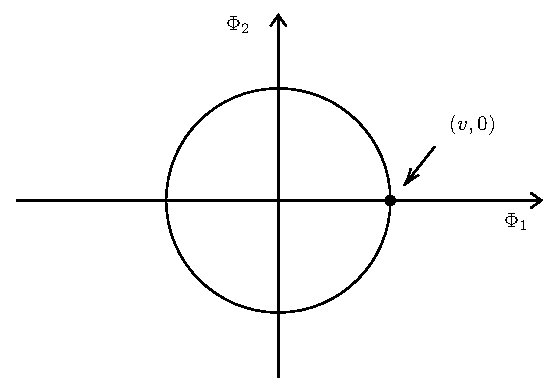
\includegraphics[width=0.55\textwidth]{../lessons/n_image/4.pdf}
\caption{\label{fig:n_4} Plane \( (\Phi _1, \Phi _2) \). The minimum lies on a circle of radius \( v = \sqrt{- \frac{r_0}{u_0}} \). }
\end{figure}


\subsubsection{Interpretation in relativistic quantum mechanics}

Now, let us give a physical interpretation of the results previously obtained and of the considerations we have done in order to obtain them. In particular:

\begin{enumerate}
\item Choosing \( r_0 <0 \) corresponds to an \emph{imaginary mass}. This is because moving away from \( \Phi =0 \), the system experiences a \emph{negative resistence} in both directions, being \( \Phi =0 \) a relative local maximum.

\item The minimum has the lowest energy and therefore it must correspond to the \emph{empty state}.
In this case, however, there is an infinite number of empty states!

\end{enumerate}

In summary, the starting Hamiltonian \( \mathcal{H} \) (or Lagrangian \( \mathcal{L} \)) is invariant with respect to \( U(1) \), but the one that describes the fluctuation dynamics around one of the chosen minimum state is not invariant with respect to \( U(1) \). Let us see in more details why the Hamiltonian, or Lagrangian, it is not invariant anymore in the case \( r_0 <0 \).

First of all, let us write the Lagrangian with respect to the fluctuations of \( \Phi _1  \)  and \( \Phi _2 \) around the chosen state \( (v,0) \) (Eq.\eqref{eq:n_7}), we obtain:
\begin{equation*}
  \begin{cases}
   \Phi _1 = v + \delta \Phi _1\\
   \Phi _2 = 0 + \delta \Phi _2
  \end{cases}
  \quad \Rightarrow \Phi = \Phi _1 + i\Phi _2 = v + \qty(\delta \Phi _1 + i \delta \Phi _2)
\end{equation*}
where we omit the factor \( 1/\sqrt{2}  \) for simplicity. Let us note that
\begin{equation*}
  \begin{cases}
   \delta \Phi _1 = \Phi _1 - v\\
   \delta \Phi _2 = \Phi _2
  \end{cases}
  \quad \Rightarrow
  \expval{\delta \Phi _1} _{\Phi _0 } = \expval{\delta \Phi _2}_{\Phi _0} = 0
\end{equation*}
indeed, as expected, the expectation value of the empty state is back to be zero.

Now, for the quantum relativistic Lagrangian \( \mathcal{L} \), let us define
\begin{equation*}
  r_0 \rightarrow m^2, \quad u_0 \rightarrow \lambda , \quad v^2 = - \frac{m^2}{\lambda }
\end{equation*}
(recall that we are still in the case \( r_0<0 \)!).
Hence, the Lagrangian Eq.\eqref{eq:n_8} becomes

\begin{equation*}
\begin{split}
\mathcal{L}  = & - \frac{1}{2} \partial _ \mu \qty(v+\delta \Phi _1 + i \delta \Phi _2)   \partial ^\mu \qty(v+\delta \Phi _1 - i \delta \Phi _2)  \\
 & - \frac{m^2}{2} \qty(v + \delta \Phi _1 + i \delta \Phi _2) \qty(v + \delta \Phi _1 - i \delta \Phi _2) \\
 & - \frac{\lambda }{4} \qty[ \qty(v + \delta \Phi _1 + i \delta \Phi _2) \qty(v + \delta \Phi _1 - i \delta \Phi _2) ] ^2 \\
 =& - \frac{1}{2} \qty(\partial_ \mu  \delta \Phi _1 \partial^ \mu \delta \Phi _1  )
 - \frac{1}{2} \qty( \partial_ \mu  \delta \Phi _2 \partial^\mu \delta \Phi _2  )  \\
 & - \frac{m^2}{2} \qty(v^2 + 2 v \delta \Phi _1 + \delta \Phi _1^2 + \delta \Phi _2^2) \\
 &- \frac{\lambda }{4} \qty(v^2 + 2 v \delta \Phi _1 + \delta \Phi _1^2 + \delta \Phi _2 ^2)^2
\end{split}
\end{equation*}
Since we have defined \( m^2 = - v^2 \lambda  \), we can rewrite it as
\begin{equation*}
\begin{split}
\mathcal{L}   = &  - \frac{1}{2} \qty(\partial_ \mu  \delta \Phi _1 \partial^ \mu \delta \Phi _1  )
- \frac{1}{2} \qty( \partial_ \mu  \delta \Phi _2 \partial^ \mu \delta \Phi _2  )
 + \frac{\lambda v^2}{2} \qty( \mathcolorbox{green!20}{v^2} + \cancel{2 v \delta \Phi _1}  +  \bcancel{\delta \Phi _1^2 + \delta \Phi _2^2})  \\
& - \frac{\lambda }{4} \qty( \mathcolorbox{green!20}{v^4} + 4 v^2 \delta \Phi _1^2
  +   \cancel{4 v^3 \delta \Phi _1}  +  \qty(\delta \Phi _1^2 + \delta \Phi _2^2)^2 + \bcancel{2 v^2 \qty(\delta \Phi _1^2 + \delta \Phi _2^2)} + 4 v \delta \Phi _1 \qty(\delta \Phi _1^2 + \delta \Phi _2^2)   )
\end{split}
\end{equation*}
Neglecting the constant terms in \( v \) (in green), finally we obtain
\begin{equation}
\begin{split}
\mathcal{L} \qty(\delta \Phi _1, \delta \Phi _2)   = &  - \frac{1}{2} \qty(\partial_ \mu  \delta \Phi _1 )^2 - \frac{1}{2} \qty(\partial_ \mu \delta \Phi _2 )^2   \\
& \mathcolorbox{yellow!40}{- \frac{2}{2} \lambda v^2 \delta \Phi _1^2} - v \lambda \delta \Phi _1 \qty( \qty(\delta \Phi _1)^2 + \qty(\delta \Phi _2 )^2  ) \\
& - \frac{\lambda }{4} \qty( \qty(\delta \Phi _1)^2 + \qty(\delta \Phi _2)^2  )^2
\end{split}
\end{equation}
Comparing it with Eq.\eqref{eq:n_8}, we note that the yellow term \( - \lambda v^2 \delta \Phi _1^2 \) indicates that the field \( \delta \Phi _1 \) (related to the transversal fluctuations) has a null empty state \( ( \expval{\delta \Phi _1}= 0 ) \) and a mass \( M \) such that (recall that \( m^2 = - \lambda v^2 = r_0 \)):
\begin{equation*}
  M^2 = 2 \lambda v^2 =  -2 r_0 = - 2m^2
\end{equation*}
Therefore, it represents a real, massive, mesonic scalar field that is physically accettable (indeed we have \( r_0<0 \)!).
However, \( \mathcal{L} \) is not any more invariant under the transformation \( \delta \Phi _1 \rightarrow - \delta \Phi _1 \), as we wanted to show! The symmetry is broken.


\begin{remark}
  Note that the field \( \delta \Phi _2 \) has no mass (there is not a term \( \propto \delta \Phi _2^2 \))! Indeed, it describes the fluctuations along the circle where the potential \( V \) is in its minimum  which imples no dynamical inertia, that implies no mass!
\end{remark}

In summary, starting with one complex scalar field \( \Phi (\va{x}) \) having mass \( m \), when \( m^2 < 0 \) one gets a real scalar field \( \delta \Phi _1 \) with mass \( M = \sqrt{- 2 m^2}  \)  and a second scalar field \( \delta \Phi _2 \) that is massless. This is called the \textbf{Goldstone boson}. Hence, we have the following theorem:

\begin{theorem}{Goldstone's theorem}{}
If a continuous symmetry is spontaneously broken and there are no long range interactions, exists an elementary excitation with zero momentum, or particle of zero mass, called Goldstone boson.

More generally, let \( \mathcal{P} \) be a subgroup of \( \mathcal{G} \) (\( \mathcal{P} \subset \mathcal{G} \)). If \( \mathcal{G} \) has \( N \) indipendent generators and \( \mathcal{P} \)  has \( M \) indipendent generators, hence, if \( \mathcal{P} \) is the new (lower) symmetry, therefore \( N-M \)  Goldstone bosons exist.
\end{theorem}

In the previous case the symmetry group was \( \mathcal{G} = U (1) \), hence \( \mathcal{G} \) has \( N=1 \) indipendent generators, whereas we have \( M=0 \) (we have chosen a specific minimum). Therefore, we have only one Goldstone boson.


\begin{example}{\(\pmb{XY}\) model}{}
Let us consider the \( XY \) model in statistical mechanics. We have that
\begin{itemize}
\item \( \delta \Phi _1 \) represents the fluctuation of the modulus of \( m \).
\item \( \delta \Phi _2 \) represents fluctuations of the spin directions, or spin waves.
\end{itemize}
\end{example}

\begin{remark}
In particle physics the presence of Goldstone bosons brings a serious problem in field theory since the corresponding particles are not observed! The resolution of this problem is given by Higgs-Englert-Brout (1964). In particular, the Higgs mechanism gives back the mass to the Goldstone particles, because the Goldstone theorem, that works well for a continuous global symmetry, can fail for local gauge theories!
\end{remark}



\section{Spontaneous symmetry breaking in gauge symmetries}

\subsection{Statistical mechanics}

In statistical mechanics, let us consider a Ginzburg-Landau model for superconductors in presence of a magnetic field (\emph{Meissner effect}, i.e. the magnetic induction \( \va{B} = 0 \) inside the superconductor). The Hamiltonian of such a system is:
\begin{equation}
  \beta \mathcal{H} (\Phi ) = \int_{}^{} \dd[d]{\va{x}} \qty[\frac{1}{2}B^2 + \abs{\qty(\va{\grad }- 2 i \va{A})\Phi  }^2 + \frac{r_0}{2} \Phi ^* \Phi
  + \frac{u_0}{4} \qty(\Phi ^* \Phi )^2 - \va{B} \vdot \va{H}]
\end{equation}
where \( \frac{B^2}{2} \) is the energy of the magnetic field \( \va{B} \) and \( \va{\grad } \rightarrow \qty[\va{\grad } + i q \va{A}]  \) is the minimal coupling.
If we have an external magnetic field \( \va{H} \), the induction field is:
\begin{equation*}
  \va{B} = \va{H} + \va{M}
\end{equation*}
For normal conductors we have \( \Phi _0 = 0 \), which implies \( \va{B} = \va{H} \), while for superconductors \( \Phi \neq 0 \) and we have a spontaneous symmetry breaking.

\subsection{Field theory analog: the Higgs mechanism for an abelian group}
Let us consider the analog of the previous system in field theory: a scalar charged mesonic fields selfinteracting and in presence of an electromagnetic field with potential quadrivector \( A_ \mu  ( \va{x}) \). We begin by applying the Higgs mechanism to an abelian\footnote{In abstract algebra, an abelian group, also called a commutative group, is a group in which the result of applying the group operation to two group elements does not depend on the order in which they are written.}, \( U(1) \)  gauge theory, to demonstrate how the mass of the corresponding gauge boson (the photon) comes about.

The \( U(1) \) gauge invariant kinetic term of the photon is given by
\begin{equation*}
  \mathcal{L}_{photon} = - \frac{1}{4} F_ {\mu  \nu } (\va{x}) F ^{ \mu \nu } (\va{x}), \qquad F_ { \mu \nu } = \partial_ \mu  A _ \nu  - \partial _ \nu  A _ \mu
\end{equation*}
That is, \( \mathcal{L}_{photon}  \)  is invariant under the transformation: \( A_\mu (\va{x}) \rightarrow A_\mu (\va{x}) - \partial_ \nu \alpha  (\va{x})  \) for any \( \alpha  \) and \( x \).
If we naively add a mass term for the photon to the Lagrangian, we have
\begin{equation*}
    \mathcal{L}_{photon} = - \frac{1}{4} F_ {\mu  \nu } (\va{x}) F ^{ \mu \nu } (\va{x}) + \frac{1}{2} m_A^2 A_\mu A^\mu
\end{equation*}
 the mass term violates the local gauge symmetry; hence, the \( U(1) \)  gauge symmetry requires the photon to be massless.

Now extend the model by introducing a complex scalar field, with charge \( q \),  that couples both to itself and to the photon. In this case, because of the presence of \( A _ \mu (\va{x}) \), we should consider a theory that satisfies symmetry \( U(1) \) locally! The Lagrangian of this model is:
\begin{equation}
  \mathcal{L} = - \frac{1}{4} F_ {\mu  \nu } (\va{x}) F ^{ \mu \nu } (\va{x})
  + \qty(D _ \mu  \Phi (\va{x}))^* \qty(D _ \mu \Phi (\va{x}))
  - V (\Phi ,\Phi ^*)
\end{equation}
where
\begin{subequations}
\begin{align*}
  D_ \mu \Phi  &= \qty(\partial_ \mu  + i q A _ \mu  ) \Phi   & \text{gauge-covariant derivative}\\
  F_ { \mu \nu } &= \partial_ \mu  A _ \nu  - \partial _ \nu  A _ \mu & \text{Field strength tensor} \\
    V (\Phi , \Phi ^*) &= \frac{m^2}{2} \Phi \Phi ^* + \frac{\lambda }{4} \qty(\Phi \Phi ^*)^2 & \text{Potential}
\end{align*}
\end{subequations}
The complex scalar field we are considering is defined again as:
\begin{equation*}
  \Phi = \frac{1}{\sqrt{2} } \qty(\Phi _1 + i \Phi _2), \quad \Phi ^* = \frac{1}{\sqrt{2} } \qty(\Phi _1 - i \Phi _2)
\end{equation*}
Hence, it is easily discerned that this Lagrangian is invariant under the gauge transformations
\begin{subequations}
\begin{align*}
     \Phi  ( \va{x} ) &\rightarrow e^{i \alpha (\va{x})} \Phi (\va{x}), \quad \Phi^*  ( \va{x} ) \rightarrow e^{-i \alpha (\va{x})} \Phi (\va{x})   \\
      A_\mu (\va{x}) &\rightarrow A_\mu (\va{x}) - \partial_ \nu \alpha  (\va{x})
\end{align*}
\end{subequations}


Let us consider again two different cases:
\begin{itemize}
\item If \( m^2 >0 \): the state of minimum energy will be that with \( \Phi =0 \) and the potential will preserve the symmetries of the Lagrangian. Then the theory is simply QED with a massless photon and a charged scalar field \( \Phi  \) with mass \( m \).

\item If \( m^2 <0 \):  the field \( \Phi  \)  will acquire a vacuum expectation value. The state of minimum energy will be that with  \( \Phi = \sqrt{- \frac{m^2}{\lambda }} \equiv v  \)    (circle of radius \( \abs{\Phi } = v \)) and the global \( U(1) \)  gauge symmetry will be spontaneously broken.
\end{itemize}

Now, let us focus on  the case \( m^2<0 \). In particular, it is convenient to parametrize \( \Phi  \) by choosing
\begin{equation*}
  \bar{\Phi }_1 = v , \quad \bar{\Phi _2} = 0
\end{equation*}
Hence, we have:
\begin{equation*}
  \Phi (x) = \qty(v + \delta \Phi _1) + i \delta \Phi _2
\end{equation*}
where \( \Phi _1 \) is referred to as the Higgs boson and \( \Phi _2 \) as the Goldstone boson. As said, they are real scalar fields which have no vacuum expecation value (\( \expval{\Phi _1}_{\Phi _0} = \expval{\Phi _2}_{\Phi _0} = 0   \)).
By inserting it in the Lagrangian and by keeping in mind that \(  m^2 = -v^2 \lambda  \), the Lagrangian transforms as
\begin{equation}
\begin{split}
  \mathcal{L} = & - \frac{1}{4} F_ {\mu \nu }F ^{\mu \nu } + \frac{1}{2} \qty(\partial_ \mu \delta \Phi _1 )^2 + \frac{1}{2} \qty(\partial _ \mu \delta \Phi _2 )^2    \\
  & -\mathcolorbox{yellow!40}{\frac{2}{2} \lambda v^2 \delta \Phi _1 ^2} + \mathcolorbox{green!20}{q^2 v^2 A_{\mu } A ^{\mu }} - \mathcolorbox{red!20}{q v A ^{\mu } \partial_ \mu \delta \Phi _2} + \text{higher order terms}
\end{split}
\label{eq:n_9}
\end{equation}
Let us give a physical interpretation of the emphasized terms:
\begin{itemize}
\item \( \lambda v^2 \delta \Phi _1^2 \) means that the field \( \delta \Phi _1 \) is massive with mass \( M = v \sqrt{2 \lambda }  \)  (\emph{Higgs boson}).

\item \( q^2 v^2 A_ \mu A ^\mu  \) means that the \emph{gauge boson}  \( A _ \mu  \), the photon, has got a mass
\begin{equation*}
  M_A^2 = 2 q^2 v^2
\end{equation*}
Note that since now \( A _ \mu  \) is massive, it has three indipendent polarization states.

\item \( q v A ^ \mu  \partial _ \mu  \delta \Phi _2  \) means that the field \( \delta \Phi _2 \) is not massive (indeed there is no term \( \propto \delta \Phi _2^2 \)) and that it is mixed with \( A_ \mu  \) (\emph{Goldstone boson}). Dynamically, this means that a propagating photon can transform itself into a field \( \delta \Phi _2 \) (the photon becomes a Goldstone boson).

\end{itemize}

Summarizing, this Lagrangian now describes a theory with a Higgs boson \( \delta \Phi _1 \) with mass \( M= v \sqrt{2 \lambda }  \), a photon of mass \( M_A = qv \sqrt{2}  \) and a massless Goldstone \( \delta \Phi _2 \).


Moreover, since \( \delta \Phi _2 \) does not seem to be a physical field it should be eliminated by a gauge transformation. Hence, the strange \( \delta \Phi _2 A^\mu  \) mixing can be removed by making the following gauge transformation:
\begin{equation*}
  A _ \mu (\va{x}) \rightarrow A _ \mu (\va{x}) - \frac{1}{q} \partial_ \mu \alpha (\va{x})
\end{equation*}
We can choose \( \alpha (\va{x}) = - \frac{1}{v} \delta \Phi _2 (\va{x}) \)
\begin{equation*}
  A _ \mu (\va{x}) \rightarrow A _ \mu (\va{x}) + \frac{1}{qv} \partial_ \mu \delta \Phi _2 (\va{x})
\end{equation*}
and the gauge choice with the transformation above is called the unitary gauge.
By inserting it in the Lagrangian Eq.\eqref{eq:n_9}, we eliminate the mixed term \( q v A ^ \mu  \partial_ \mu  \delta \Phi _2  \), in red, and the term \( \frac{1}{2} \qty(\partial _ \mu  \delta \Phi _2 )^2  \). Thus we obtain:
\begin{equation}
  \mathcal{L} = - \frac{1}{4} F _{\mu \nu } F ^ {\mu \nu } + \frac{1}{2} \qty(\partial _ \mu  \delta \Phi _1 )^2 - \lambda v^2 \delta \Phi _1^2
  + q^2 v^2 A_ \mu A ^ \mu  + \text{higher order terms}
  \label{eq:n_10}
\end{equation}
The Goldstone \( \delta \Phi _2 \)  will then completely disappear from the theory and one says that the Goldstone has been "eaten" to give the photon mass.
Therefore, the new Lagrangian in Eq.\eqref{eq:n_10} contains two fields: one is a massive photon with spin 1 and the second field \( \delta \Phi _1 \) is massive too, but has spin 0 (scalar).
The mechanics trough which the gauge boson becomes massive is the so called \textbf{Higgs mechanism}.

It is instructive to count the degrees of freedom (dof) before and after spontaneous symmetry broken has occurred. In particular, we have:

\begin{itemize}
\item For a global \( U(1) \)  symmetry, we have \( 2 \) massive scalar fields, hence there are \( 1+1 \) degrees of freedom.

After symmetry breaking, we have \( 1 \)  scalar field massive and \( 1 \) scalar field not massive. Hence, there are again \( 1+1 \) degrees of freedom.

\item For a local gauge \( U(1) \) symmetry, we have \( 2 \) massive scalar fields and one massless photon. Hence, there are \( 2 + 2 \) degrees of freedom (the massless photon has \( 2 \) polarizations).

After symmetry breaking, we have \( 1 \) massive scalar field  and \( 1 \) massive photon. Hence, there are  \( 1+3 \) degrees of freedom (the massive photon has \( 3 \) polarizations).

\end{itemize}



\begin{remark}
  Let us note that in Eq.\eqref{eq:n_10} among the higher order terms we have neglected, there are
\begin{itemize}
\item A term proportional to \( \propto \delta \Phi _1 A_ \mu A ^ \mu  \), shown in Figure \ref{fig:n_7}.
\item A term proportional to \( \propto \delta \Phi _1 ^2 A _ \mu A ^ \mu  \), shown in Figure \ref{fig:n_8}.
\end{itemize}
\end{remark}

\begin{figure}[h!]
\begin{minipage}[c]{0.5\linewidth}
\subfloat[][Feyman diagram of the term \( \propto \delta \Phi _1 A_ \mu A ^ \mu  \). ]{ 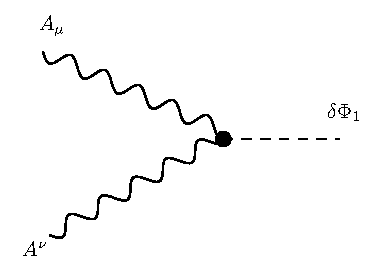
\includegraphics[width=0.8\textwidth]{../lessons/n_image/5.pdf}  \label{fig:n_7} }
\end{minipage}
\begin{minipage}[]{0.5\linewidth}
\centering
\subfloat[][Feyman diagram of the term \( \propto \delta \Phi _1 ^2 A _ \mu A ^ \mu  \).]{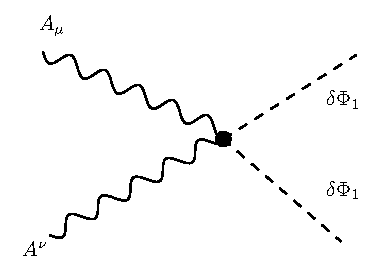
\includegraphics[width=0.8\textwidth]{../lessons/n_image/6.pdf}  \label{fig:n_8} }
\end{minipage}
\caption{\label{fig:} }
\end{figure}


\begin{remark}
Note that the  presence of the massive photon \( M^2_A = 2 q^2 v^2 \), with \( q = 2 l \) in superconductivity, gives rise to the exponential drop
\begin{equation*}
  B (x) = B(0) e^ {- x/l}
\end{equation*}
inside the system.
\end{remark}

Now, let us do some considerations:

\begin{itemize}
\item As said, we cannot introduce by hand a massive photon i.e. a term like \( \frac{1}{2} M_A^2 A_ \mu A ^\mu  \) in the Lagrangian because we would violate explicitely the gauge symmetry!
\item The Lagrangian is gauge invariant.
\item Symmetry breaking occurs at the level of the vacuum state.
\item A gauge symmetry that is explicitely broken is not renormalizable.
\end{itemize}





\subsection{Non abelian gauge theories}
Let us illustrate some examples of non abelian gauge theories.

\begin{example}{}{}
The electro-weak interactions theory (Glashow-Weinberg-Solam) (theory of leptons) is a non abelian gauge theories: the Lagrangian is invariant under the group \( \underbrace{S U (2)}_{\substack{ \text{weak} \\  \text{interactions} } }  \times \underbrace{U(1)}_{\text{electromagnetism}}  \), that is not an abelian group because of \( S U(2) \).
\end{example}

\begin{example}{Quantum chromodynamic (quarks+gluons)}{}
In the case of quantum chromodynamic, one has a term that is \( SU(3) \) invariant and the GWS Lagrangian that has symmetry \( SU(2) \times U(1) \). It implies that the Lagrangian of this theory is invariant under
  \begin{equation}
    SU(3) \times SU(2) \times U(1)
  \end{equation}
Because of the groups \( SU(2) \) and \( SU(3) \) the symmetries above ar not abelian (for example in \( SU(2) \) two matrices \( U (\alpha ) \) and \( U(\beta ) \) do not commute in general).
\end{example}


\subsection{Extension of Higgs mechanism to non abelian theories}

\subsection{GWS model}
Complex field \( SU(2) \)
\begin{equation}
  \Phi = \frac{1}{\sqrt{2} } \begin{pmatrix}
  \Phi _1 + i \Phi _2 \\
  \Phi _3 + i \Phi _4
  \end{pmatrix}
  =
  \begin{pmatrix}
  \Phi _a (\va{x}) \\
  \Phi _b (\va{x})
  \end{pmatrix}
\end{equation}
where \( \Phi _a, \Phi _b \) are complex fields.

Gauge transformation \( SU(2) \times U(1) \):
\begin{equation}
  \begin{pmatrix}
  \Phi _a (\va{x}) \\
  \Phi _b (\va{x})
  \end{pmatrix}
  \rightarrow
  e^{\frac{i}{2} \alpha _0 (\va{x})} e^{\frac{i}{2} \va{\tau } \vdot \va{\alpha } (\va{x})}
  \begin{pmatrix}
  \Phi _a (\va{x}) \\
  \Phi _b (\va{x})
  \end{pmatrix}
\end{equation}
where \( \va{\tau } \) are Pauli matrices, \( \alpha _0, \alpha _1, \alpha _2, \alpha 3 \) are four real functions (4 vectorial mesons).
\begin{equation}
  \va{\alpha } (\va{x}) \rightarrow W _ \mu ^ a (\va{x}) = \qty( W_ \mu ^{(1)} (\va{x}),  W_ \mu ^{(2)} (\va{x}),  W_ \mu ^{(3)} (\va{x}) )
\end{equation}
The scalar gauge field is
\begin{equation}
  \alpha _0 (\va{x}) \rightarrow B _ \mu (\va{x})
\end{equation}
with \( B _ \mu  \) is a linear combination of \( A_ \mu  \) and \(  W_ \mu ^{(3)}  \).

Lagrangian:
\begin{equation}
  \mathcal{L} = \qty(D_ \mu \Phi )^\dagger \qty(D ^ \mu \Phi ) - \mu ^2 \Phi ^* \Phi - \lambda \qty(\Phi ^* \Phi )^2
  - \frac{1}{4} b^{\mu \nu } b_{\mu \nu } - \frac{1}{4} f_a^{\mu \nu } f_{\mu \nu }^a
\end{equation}
\begin{equation}
  D_ \mu  \rightarrow \partial_ \mu \frac{1}{2} i g \tau ^a W_ \mu ^a - \frac{i}{2} g' B _ \mu
\end{equation}
\begin{equation}
  f_ {\mu \nu }^a = \partial_ \mu W_ \nu ^a - \partial_ \nu W _ \mu ^a - g \varepsilon ^{abc} W _ \mu ^b  W_ \nu ^a
\end{equation}
\begin{equation}
  b_ {\mu \nu } = \partial_ \mu B _ \nu - \partial_ \nu  B _ \mu
\end{equation}
\begin{subequations}
\begin{align}
  W_ \mu ^a & \rightarrow W_ \mu ^a - \varepsilon ^{abc} \alpha _b (\va{x}) W_ \mu ^c (\va{x}) + \frac{1}{g} \partial_ \mu \alpha ^a (\va{x})    \\
  B _ \mu  & \rightarrow  B _ \mu + \frac{1}{g'} \pdv{\alpha _0}{x_ \mu }
\end{align}
\end{subequations}
\begin{equation}
  \nu \sim \Phi _1^2 + \Phi _2^2 + \Phi _3^2 +\Phi _4^2 = v^2
\end{equation}
Choosing the direction on the sphere in \( \R^4 \), 3 symmetries are broken a 3 Goldstone bosons.

\subsection{Higgs mechanism}
Higgs scalar field
\begin{equation}
  \delta \Phi = \begin{pmatrix}
  \Phi ^+ \\
  \Phi _0
  \end{pmatrix}
\end{equation}
such that
\begin{equation}
  \bra{0} \Phi \ket{0} = \begin{pmatrix}
  0 \\
  v
  \end{pmatrix}
\end{equation}
\begin{equation}
  \Rightarrow \mathcal{L}_{Higgs} = \frac{1}{2} (g \nu )^2 W_ \mu ^+ W^{- \mu }
  + \frac{1}{2} v^2 \qty(g W _ \mu ^{(3)} - g' B _ \mu )^2
\end{equation}
where
\begin{subequations}
\begin{align}
  W_ \mu ^{(1)} &=  \frac{1}{\sqrt{2} } \qty(W_ \mu ^+ + W _ \mu ^-) \\
  W_ \mu ^{(2)} &=  \frac{1}{\sqrt{2} } \qty(W_ \mu ^+ - W _ \mu ^-)
\end{align}
\end{subequations}
Mass of the \( W^+ \) particle and its antiparticle
\begin{equation}
  M_W^2 = \frac{1}{2} \qty(g v)^2
\end{equation}
The \( 2^{nd} \) term is a linear combination of \( W_ \mu ^3 \) and \( B_ \mu  \) which corresponds to \( Z^0 \), the field for a third weak gauge boson.

To make \( Z_ \mu ^0 \) and \( A _ \mu  \) orthogonal we should consider
\begin{subequations}
\begin{align}
  A_ \mu  &=  \qty(\cos \theta _W) B _ \mu  + \qty(\sin \theta _W ) W_ \mu ^3 \\
  Z_ \mu ^0 & = \qty(- \sin \theta _W ) B _ \mu + \qty(\cos \theta _W ) W_ \mu ^3
\end{align}
\end{subequations}
where \( \theta _W \) is the Weiberg angle:
\begin{equation}
  \tan \theta _W = \frac{g'}{g}
\end{equation}
\begin{equation}
  M_ {Z^0}^2 = \frac{1}{2} \qty(\frac{vg}{\cos \theta _W})^2 = \frac{M w^2}{\cos^2 \theta _W}
\end{equation}



\end{document}
